\documentclass{arduino}
\usepackage{lipsum}
\setmainlanguage{dutch}
\graphicspath{{images/}}

\begin{document}

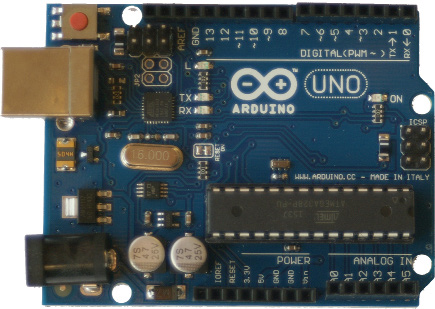
\includegraphics[width=6cm]{1. Arduino}

\textbf{Benodigdheden voor deze module}

\begin{tabular}{l}
Arduino \\
Breadboard \\
Jumperkabels \\
Weerstanden (\SI{220}{\ohm}; \SI{330}{\ohm}; \SI{1}{\kilo\ohm}; \SI{10}{\kilo\ohm}) \\
Potmeter (\SI{1}{\kilo\ohm}; \SI{10}{\kilo\ohm}) \\
Diode \\
2x LDR \\
LED (rood, geel, groen) \\
RGB LED \\
Servo motor \\
DC Motor \\
5x Drukknop \\
2N2222 transistor \\
LCD \\
Actieve piëzo element \\
\end{tabular}

\textbf{Benodigde voorkennis}

\begin{tabular}{ll}
Wet van Ohm & $R = \dfrac{U}{I}$\\
Serieschakeling & stroomsterkte gelijk \\
Parallelschakeling & spanning gelijk \\
Vermogen & $P = U \cdot I = I^2 \cdot R$ \\
\multicolumn{2}{l}{Werking dynamo/elektromotor}\\
\end{tabular}

\newpage

\section{Introductie}

\marginfigure[\baselineskip]{2. Aurduino - welcome}
Leuk dat je aan de slag gaat met Arduino! Wellicht heb je nog geen idee wat een Arduino is en wat je er mee kunt. Een Arduino is een soort microcomputer. De Arduino sluit je aan op een computer waarbij je een programma (in Arduino noemen ze dat een sketch) stuurt naar de Arduino. De Arduino voert vervolgens je geschreven script uit en zorgt voor de uitvoer. Zo kun je een koelkast op een bepaalde temperatuur houden, een zelfrijdende robot aansturen, lichtsensoren maken, een lcd scherm op je shirt aansturen en ga zo maar door. Ook is het mogelijk om geen software te gebruiken en alleen met de elektronica te spelen. De Arduino is dan de spanningsbron.

In deze module gaan we aan het werk met de Arduino en leren we de basismogelijkheden van een Arduino. Bij het werken met een Arduino heb je twee belangrijke onderdelen: De Arduino en een breadboard. De Arduino is de computer, met invoer en uitvoer mogelijkheden. Op het breadboard sluit je de elektronica aan die aangestuurd wordt door de Arduino.

\subsection{Breadboard}

\marginfigure[\baselineskip]{3. Arduino - breadboard}
\marginfigure[\baselineskip][0.5]{4. Breadboard}
Het breadboard heeft aan beide zijdes twee kolommen die verbonden worden met de voeding (+ en -). De + kant sluit je aan op de \SI{5}{\volt} uitgang of op een uitvoerpoort van de Arduino. De – kant sluit je aan op de GND (ground) van de Arduino. Alhoewel je de constante output niet altijd gebruikt, is het wel verstandig om deze altijd aan te sluiten.

Het breadboard heeft rijen en kolommen, zie hiernaast en hieronder voor een opgewerkte breadboard. De punten in een rij zijn met elkaar verbonden. Maar laten we hier niet te lang bij stil staan\dots we gaan aan de slag!

\textbf{NB:} Vaak moet je even aangeven in welke USB-Poort je Arduino zit. Dit doe je door in het programma te gaan naar: Hulpmiddelen/Poort. Daar kun je de juiste USB poort aanklikken.


\newpage

\subsection{Opdracht 1 Het aansluiten van een LED}

\begin{minipage}[m]{0.6\textwidth}
Een LED is een diode die licht uitzendt als er stroom door de LED gaat. De LED laat stroom maar door in één richting. De lange poot van de LED moet altijd op de + kant aangesloten worden, de korte poot op de – kant, zie onderstaand figuur.

De stroom door een LED mag meestal maar \SI{20}{\milli\ampere} zijn. De spanning over de LED is dan ongeveer \SI{2.0}{\volt}, deze waardes verschillen een beetje per soort LED, zie onderstaande tabel. De Arduino levert een \SI{5.0}{\volt} spanning. De LED moet dus in serie geschakeld worden met een weerstand. De weerstand moet dus minimaal \SI{150}{\ohm} zijn ($R = \frac{U}{I} = \frac{\SI{3.0}{\volt}}{\SI{0.020}{\ampere}} = \SI{150}{\ohm}$).
\end{minipage}\hfill\begin{minipage}[m]{0.39\textwidth}
\raggedleft
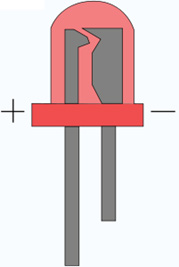
\includegraphics[width=1.5cm]{5. Component LED}
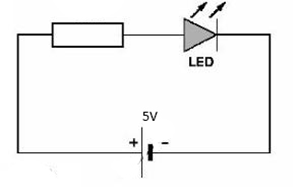
\includegraphics[width=5cm]{6. LED circuit}
\end{minipage}

\begin{minipage}[m]{0.6\textwidth}
\begin{enumerate}[label={\alph*})]
\item Er is geen weerstand aanwezig van \SI{150}{\ohm} maar wel een van \SI{220}{\ohm}. Zoek de weerstand op met behulp van de kleurcode: de eerste ring moet rood zijn, de tweede ring ook en de derde ring bruin ($\textcolor{red}{2}\textcolor{red}{2} \cdot \textcolor{brown}{10}$). Een andere mogelijkheid is rood, rood, zwart, zwart ($\textcolor{red}{2}\textcolor{red}{2}\textcolor{black}{0} \cdot \textcolor{black}{1}$).

\item Sluit nu de \SI{5}{\volt} uitgang van de Arduino aan op de + kolom en de GND (ground) uitgang van de Arduino aan op de – kolom.

\item Sluit de LED en de weerstand in serie aan, zie de tekening.

\item Verbind de Arduino via de usb met de computer. Als je het goed hebt gedaan brandt de LED!
\end{enumerate}

Doordat de rode led bij lagere spanning licht uit zendt dan bijvoorbeeld een groene led, kun je een kleinere weerstand bij groene en blauwe led’s gebruiken. Zo branden ze uiteindelijk toch nog even fel!

\begin{tabular}{ll}
\textbf{Kleur} & \textbf{Drempelspanning}\\
Blauw & \SI{2.3}{\volt} \\ 
Groen & \SI{2.0}{\volt} \\
Rood  & \SI{2.0}{\volt} \\
\end{tabular}
\end{minipage}\hfill\begin{minipage}[m]{0.39\textwidth}
\raggedleft
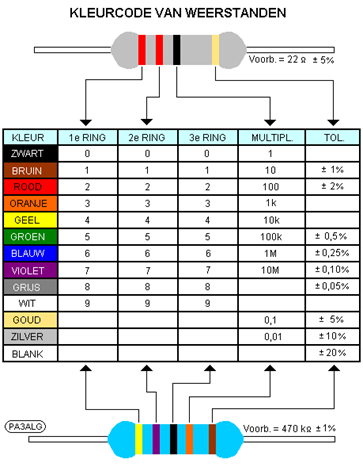
\includegraphics[width=6cm]{7. Component resistor values}
\smallskip
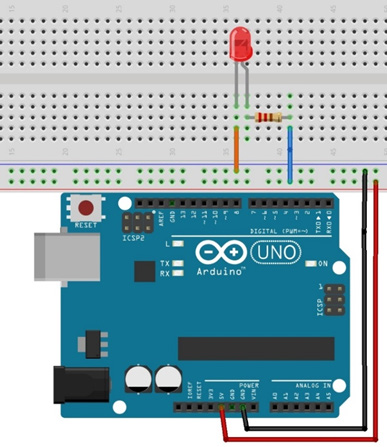
\includegraphics[width=6cm]{8. Circuit switchable LED}
\end{minipage}


\subsection{Opdracht 2 Een knipperende LED}

\begin{wrapfigure}{R}{8cm}
\raggedleft
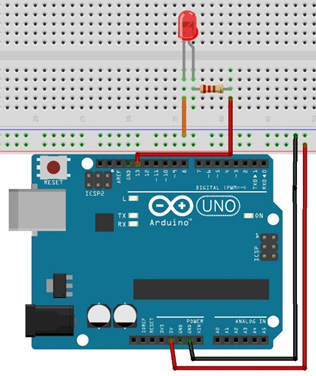
\includegraphics[width=6cm]{9. Circuit blinking LED}

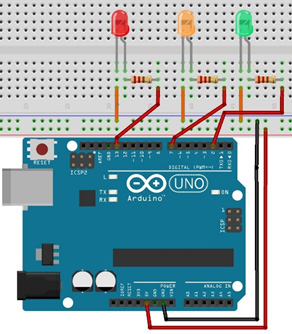
\includegraphics[width=6cm]{11. Circuit traffic light}
\end{wrapfigure}

Nu kun je je led wel laten branden, maar daar heb je nog niet veel aan\dots Een volgende stap is de LED aansturen met behulp van een stukje code. Om de LED aan te sturen met behulp van code moet je een uitvoerpoort (bijvoorbeeld pin 13) van de Arduino verbinden met je LED. De \SI{5}{\volt} output heb je nu niet nodig, pin 13 levert nu de spanning. In de tekening zie je dat deze wel verbonden is, bij grotere projecten vergeet je snel de \SI{5}{\volt}, vandaar!

\begin{enumerate}[label={\alph*})]
\item Bouw de opstelling die je ziet in de tekening en sluit de Arduino aan op de computer.
\end{enumerate}

We willen de Arduino aansturen, daarvoor gebruiken we het Arduino programma.

\begin{enumerate}[label={\alph*})]
\item Open het programma en open het script blink via: bestand/voorbeelden/basis/blink.

\item Controleer het script met het vinkje. Mocht het programma niet werken, dan geeft het onderaan een foutmelding weer (het kan zijn dat je de COM-poort moet toewijzen, dit doe je via hulpmiddelen/poort).

\item Upload het script naar je Arduino met het tekentje 
\includegraphics{10. Arduino upload} (snelcode: ctrl + u)

\item Beschrijf kort wat je ziet. Probeer wat je ziet te verklaren met behulp van de code.

\item Verander het script zodat de LED sneller knippert.

\item Sluit drie verschillende LED lampjes aan, verander het script zodat ze om de beurt aan staan.

\item Verander het script en maak een verkeerslicht waarbij oranje maar even aan staat.
\end{enumerate}

\section{Programmeren deel 1}

\begin{wrapfigure}{R}{11cm}
\raggedleft
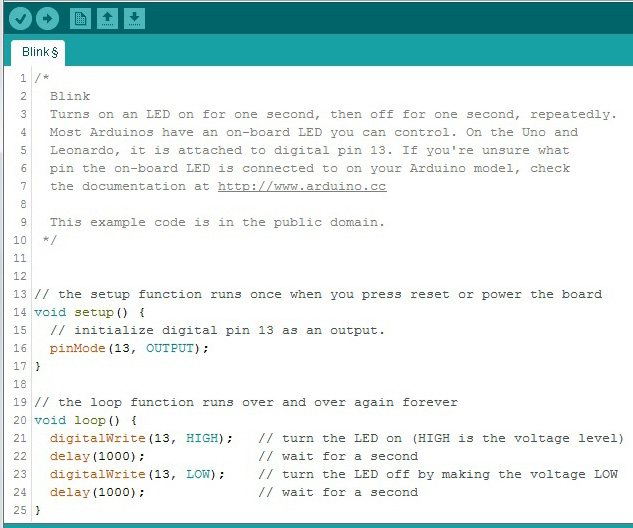
\includegraphics[width=9.5cm]{12. Arduino code}
\end{wrapfigure}

Arduino heeft een eigen programma dat gebaseerd is op C++. Heb je al ervaring met programmeren en/ of met C++ (of java), dan is het programmeren heel makkelijk. Heb je geen ervaring met programmeren? Het is veel minder moeilijk dan je misschien wel denkt!

Bovenaan het script Blink staat /* dit betekent dat alles na dit beginteken en voor het afsluitteken */ commentaar is. Hier zet je neer hoe het programma heet, wat het doet, wie het gemaakt heeft en wanneer je het voor het laatst hebt veranderd.

\begin{lstlisting}
void setup(){
  pinMode(13,OUTPUT);
}
void loop() {
  digitalWrite(13, HIGH);
  delay(1000);
  digitalWrite(13, LOW);
  delay(1000);
}
\end{lstlisting}

Een tweede mogelijkheid om commentaar toe te voegen is met behulp van //. Alles op dezelfde regel na // is commentaar. Zo kun je bijhouden wat de code op die regel doet. Met behulp van de snel code ctrl / kun je code snel omzetten naar commentaar.

Voordat de belangrijkste code wordt uitgevoerd moet je zeggen wat er precies aangestuurd wordt. We geven aan dat in pin 13 iets zit en dat de Arduino daar een output (spanning) geeft als jij dat wilt. Iets netter zou zijn om nog voor de setup aan te geven hoe pin 13 heet: je geeft de pin een naam (\lstinline{int} LEDrood = 13;). Wil je pin 13 vervolgens aansturen, dan kan je dat doen met de naam LEDrood.

Alles wat tussen de accolades {} van de loop staat wordt continu herhaald. Eerst wordt pin 13 hoog (\SI{5.0}{\volt}) gemaakt met behulp van de code \lstinline{digitalWrite} (\lstinline{digitalWrite} kan alleen aan of uit). Daarna moet het programma \SI{1000}{\milli\s} wachten (delay) voordat de volgende regel code wordt uitgevoerd. De volgende regel code maakt pin 13 weer laag (\SI{0.0}{\volt}).

\begin{wrapfigure}{R}{8cm}
\raggedleft
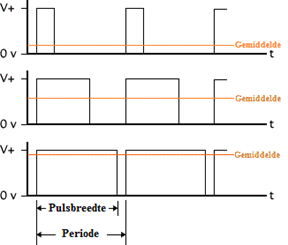
\includegraphics[width=6cm]{13. PWM}
\end{wrapfigure}

De pin wordt aangestuurd met een hoog of met een laag signaal. Zit daar nog iets tussen? Ja en nee\dots De output is altijd \SI{0.0}{\volt} of \SI{5.0}{\volt}. Maar je kunt de LED wel dimmen door maar een bepaalde tijd de LED aan te zetten. Als de LED snel genoeg knippert zie je niet dat de LED knippert, het lijkt er alleen op dat de LED minder fel brandt. Wanneer je een LED wilt dimmen gebruik je een output met het symbool $\sim$. Dit is een Puls Width Modulation (PWM). De waarde van de PWM zit tussen de 0 (geheel uit) en 255 (geheel aan).


\subsection{Opdracht 3 Een LED dimmen}

\begin{wrapfigure}{R}{8cm}
\raggedleft
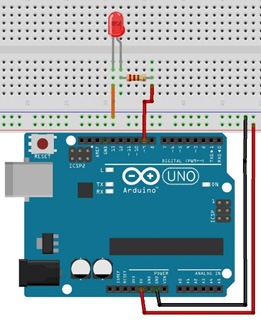
\includegraphics[width=6cm]{14. Circuit dimmable LED}
\end{wrapfigure}

\begin{enumerate}[label={\alph*})]
\item Bouw de opstelling die hiernaast staat.  Gebruik bij de output een PWM pin, bijvoorbeeld Pin 9 (let op, de LED hoeft niet aangesloten te worden aan de constante spanning, de spanning wordt nu geleverd door pin 9).

\item Open het script Fade in de voorbeelden/basis en upload het script.

\item Beschrijf wat je ziet en probeer met behulp van de code een te verklaren wat er gebeurt.

\item Verander de code zodat de LED sneller volledig brandt en sneller uit is. Let op, er zijn twee manieren! Probeer ze allebei uit.

\item In de code staat \lstinline{analogWrite}. Voorheen hebben we \lstinline{digitalWrite} gebruikt. Leg uit waarom dat nu niet kan.
\end{enumerate}

\subsection{Opdracht 4 Een aan en uit knop voor de LED}

\begin{wrapfigure}{R}{8cm}
\raggedleft
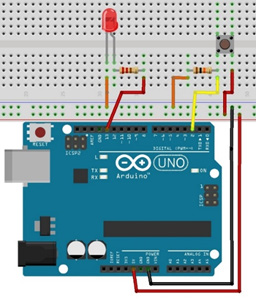
\includegraphics[width=6cm]{15. Circuit LED button}
\end{wrapfigure}

We kunnen nu de LED met behulp van de code aan en uit zetten en zelfs dimmen. Maar vaak wil je ook een schakeling handmatig aan en uit kunnen zetten. Daarvoor hebben we een drukknop nodig.

\begin{enumerate}[label={\alph*})]
\item Bouw de schakeling die hiernaast staat. Let op dat je een grote weerstand gebruikt zodat de te leveren stroom niet te groot is, een Arduino is namelijk slecht in het leveren van grote stroomsterktes.
\end{enumerate}

Het idee is nu dat we pin 2 gebruiken als INPUT. Pin 2 meet de spanning op dat punt (vergelijkt deze met \SI{0.0}{\volt}). Dit gebeurt met de code digitalRead(). Deze kan nu een hoog (\SI{5.0}{\volt}) of laag (\SI{0.0}{\volt}) signaal meten (met een analoge pin, A0 t/m A5, kunnen ook tussen gelegen waardes (10 bits) gemeten worden). Pin 2 meet alleen een spanning als de knop (button) ingedrukt wordt.

\begin{enumerate}[label={\alph*})]
\item Open het script Button via voorbeelden/digitaal en upload het script.

\item Druk op de knop en controleer wanneer de LED uit is en wanneer deze aan is.

\item Pas het script aan zodat de functie van de knop precies omgedraaid wordt.
\end{enumerate}

\begin{wrapfigure}{R}{8cm}
\raggedleft
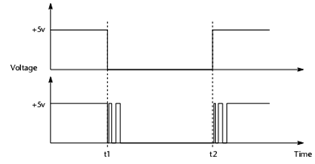
\includegraphics[width=6cm]{16. Button bounce}
\end{wrapfigure}

\textbf{NB:} Met de button is er iets bijzonders aan de hand. Deze heeft namelijk een zogenaamde Bounce. Dit betekent dat de spanning niet direct van \SI{0}{\volt} naar \SI{5}{\volt} gaat maar, nog een keer op en neer gaat. Dit komt omdat er in de button een veer zit die op en neer gaat. Bij het gebruik en uitlezen van de button is het dus handig om een delay in te bouwen\dots

\section{Programmeren deel 2}

Het script Button is uitgebreider dan we voorheen hebben gezien. We lopen stap voor stap door het script.

\begin{lstlisting}
const int buttonPin = 2;
const int ledPin = 13;
\end{lstlisting}

We hebben te maken met twee poorten waar iets moet gebeuren. Pin 2 is een invoer en pin 13 moet een uitvoer zijn. De pin verandert niet, dit is een constante (\lstinline{const}). Het is een gehele waarde, een integer (\lstinline{int}). We geven pin 2 een herkenbare naam, pin 2 heet nu buttonPin. Pin 13 heeft de naam ledPin gekregen.

\begin{lstlisting}
int buttonState = 0;
\end{lstlisting}

We willen straks weten wat de ‘staat’ van de knop is (ingedrukt of niet). Deze kan 1 of 0 zijn. We moeten even vertellen dat we de staat van de knop willen weten (aanmaken van een variabele) en deze straks willen vergelijken. Voordat we het script laten draaien is de buttonState gelijk aan 0.

\begin{lstlisting}
void setup() {
  pinMode(ledPin, OUTPUT);
  pinMode(buttonPin, INPUT);
}
\end{lstlisting}

Zoals gezegd, we moeten even vertellen dat de ledPin een \lstinline{OUTPUT} is en de buttonPin een \lstinline{INPUT}. Zo, dat weten ze nu dan ook\dots

Er moet iets gebeuren als de knop wordt ingedrukt. Aan het begin van de loop wordt de knop uitgelezen
(eigenlijk wordt er alleen gecontroleerd of er een
\SI{5.0}{\volt} spanning over de weerstand staat). Daarna volgt een if-statement. Als (\lstinline{if}) de knop is ingedrukt (\lstinline{buttonState == HIGH}) dan moet de LED gaan branden (\lstinline{digitalWrite(ledPin, HIGH);}). In alle andere gevallen (\lstinline{else}), moet de LED niet branden (\lstinline{digitalWrite(ledPin,LOW);}).

\begin{lstlisting}
void loop() {
  buttonState = digitalRead(buttonPin);
  if (buttonState == HIGH) {
    digitalWrite(ledPin, HIGH);
  }
  else {
    digitalWrite(ledPin, LOW);
  }
}
\end{lstlisting}

\begin{lstlisting}
void loop() {
  buttonState = digitalRead(buttonPin);
  if (buttonState == HIGH && state == LOW) {
    state2 = HIGH;
    }
  if (buttonState == HIGH && state == HIGH) {
    state2 = LOW;
    }
  state = state2;
  digitalWrite(ledPin,state);
  delay (100);
}
\end{lstlisting}

\begin{lstlisting}
if(buttonState == HIGH){i++;}
digitalWrite(ledPin,i%2);
\end{lstlisting}

Het is een makkelijk if-statement. Je kunt ook meerdere voorwaarden stellen. Als je twee knoppen tegelijk in moet drukken voordat de LED gaat branden zet je \&\& tussen de tekens (\lstinline{if buttonState1 == HIGH && buttonState 2 == HIGH)}).%{}
Je kunt ook het teken || gebruiken. Dan moet of de ene voorwaarde gelden of de andere. Helaas blijft het lampje nu nog niet branden als je de knop hebt ingedrukt. Je kunt er wel zelf voor zorgen dat je met één knop het lampje aan en uit kan zetten. 

Vergeet niet de nieuwe variabele (\lstinline{int}) te definiëren aan het begin! Er zijn nog eenvoudigere manieren, deze zijn alleen getoond als script. Leg uit hoe ze werken! 

\begin{lstlisting}
digitalWrite(13,!digitalRead(13));
\end{lstlisting}

\subsection{Opdracht 5 Het beveiligen van een kluis}

De kluis van de bank is beveiligd. De kluis gaat pas open (de LED brandt pas) als er twee sleutels worden omgedraaid (knoppen ingedrukt). Een sleutelgat bevindt zich op de kamer van de directeur, de andere zit naast de kluis.

Bouw de bijbehorende schakeling en programmeer het script zodanig dat de kluis pas open gaat als beide sleutels tegelijk worden omgedraaid.

\subsection{Opdracht 6 Een wisselschakeling}

Als je onderaan de trap staat wil je het licht bovenaan de trap aan zetten. Bovenaan de trap zit nog een lichtknop. Daarmee kan je het licht weer uit of aan zetten. Bouw de schakeling met twee knoppen en schrijf het programma zodat je een werkende wisselschakeling hebt. Lukt dit niet meteen? Probeer het dan eerst met een enkele knop. 

\subsection{Opdracht 7 Een voetgangersoversteekplaats}

Voor voetgangers is een speciale overgangsplek gemaakt. Deze plek ligt aan een drukke weg. Als er geen voetgangers zijn, staat het verkeerslicht voor de auto’s op groen. Op het moment dat een voetganger over wil steken, drukt deze op de knop. Het verkeerslicht voor de auto’s gaat dan van groen naar geel naar rood. Voetgangers hebben dan 15 seconde om over te steken. Het verkeerslichtvoor hen staat op groen! Dan gaat het groene lampje vijf keer knipperen en springt op rood. Een seconde later springt het verkeerslicht voor de auto’s weer op groen. 

Maak dit systeem.

% \section{Elektronica deel 1}

% \begin{wrapfigure}{R}{8cm}
% \raggedleft
% 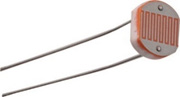
\includegraphics[width=4cm]{17. Component LDR}

% 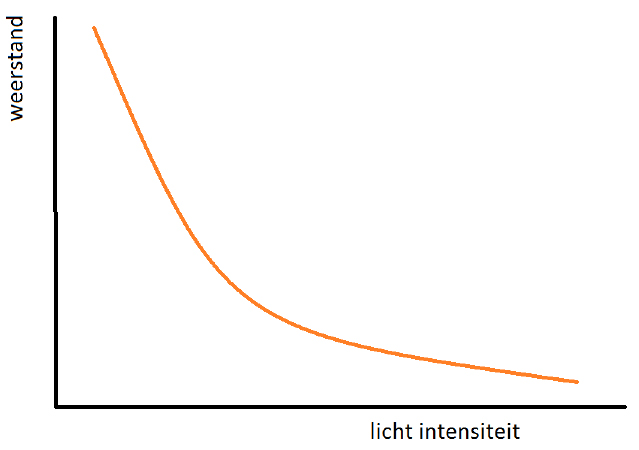
\includegraphics[width=6cm]{18. LDR resistance vs light intensity}
% \end{wrapfigure}

% Wanneer je alleen een knop en een LED gebruikt ben je snel uitgekeken en heb je nog nauwelijks iets gedaan\dots We willen robots aansturen, racemachines niet tegen muren laten botsen, kassen automatisch aansturen en ga zo maar door. Daar hebben we sensoren voor nodig. Vrijwel alle sensoren werken hetzelfde, de weerstandswaarde verandert bij een veranderende input (bijvoorbeeld licht of kracht). We gaan beginnen met een lichtsensor. Voor een lichtsensor hebben we een LDR nodig, zie de foto. LDR staat voor Light Dependent Resistor (licht afhankelijke weerstand). De weerstandswaarde verandert met veranderende lichtintensiteit, zie de grafiek.

% \begin{wrapfigure}{R}{8cm}
% \raggedleft
% 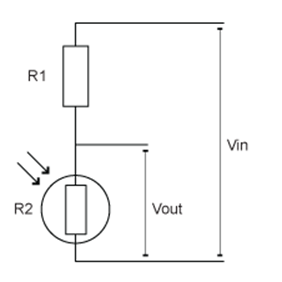
\includegraphics[width=4cm]{19. LDR circuit}
% \end{wrapfigure}

% We sluiten de LDR in serie aan met een Ohmse weerstand (een weerstand met een constante weerstandswaarde). Zo hebben we een spanningsdeler gemaakt. Een deel van de spanning staat over de LDR en een deel van de spanning staat over de weerstand. Het enige wat we moeten doen is de spanning over de LDR uitlezen en we weten hoe licht het is!

% Het is belangrijk om iets meer te weten over hoe een spanningsdeler werkt: bij het uitlezen van een sensor maken we gebruik van een spanningsdeler. De LDR en de Ohmse weerstand staan in serie zodat er geldt: $R_\mathrm{totaal} = R_\mathrm{LDR} + R_{\si{\ohm}}$. De bronspanning is \SI{5.0}{\volt} en omdat de   weerstanden in serie geschakeld zijn geldt dat de stroomsterkte overal gelijk is. De stroomsterkte bereken je met: $I = \dfrac{U_\mathrm{bron}}{R_\mathrm{totaal}}$. De spanning wordt netjes verdeeld en de grootste weerstand krijgt de meeste spanning. Als je deze informatie combineert zie je dat de verhouding tussen de spanningen gelijk is aan de verhouding tussen de weerstanden: $\dfrac{U_\mathrm{LDR}}{U_{\si{\ohm}}} = \dfrac{R_\mathrm{LDR}}{R_{\si{\ohm}}}$.

% \begin{wrapfigure}{R}{10cm}
% \raggedleft
% 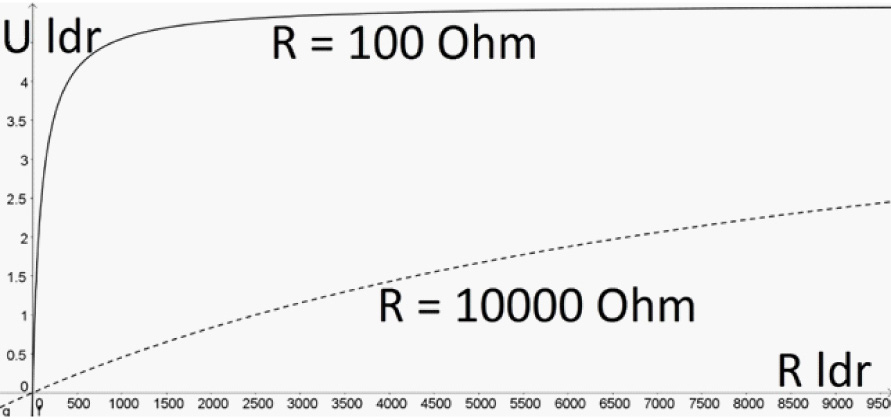
\includegraphics[width=8cm]{20. LDR potantial vs resistance}
% \end{wrapfigure}

% Als het lichter is, wordt de weerstandswaarde van de LDR kleiner waardoor er minder spanning over de LDR staat maar meer spanning over de Ohmse weerstand. De spanning over de LDR ($U_\mathrm{LDR} = \SI{5.0}{\volt} \cdot \dfrac{R_\mathrm{LDR}}{(R_\mathrm{LDR} + R_{\si{\ohm}})}$ kun je meten met behulp van de ANALOG IN van de Arduino. De spanning is dan een maat voor de gemeten lichtintensiteit. 

% In welk gebied je sensor gevoelig moet zijn bepaalt de keuze voor een Ohmse weerstand. Zie de tweede grafiek. De LDR heeft een waarde tussen de \SI{10}{\kilo\ohm} en \SI{20}{\kilo\ohm}: dus kies een grote weerstand!


% \subsection{Opdracht 8 Een lichtsensor}

% \begin{wrapfigure}{R}{10cm}
% \raggedleft
% 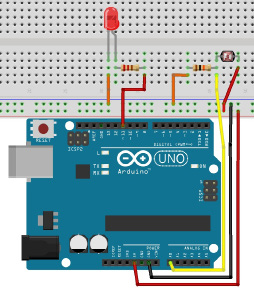
\includegraphics[width=8cm]{21. Circuit light sensor}
% \end{wrapfigure}

% De schakeling lijkt erg op de schakeling van opdracht 4. Alleen nu gebruiken we een LDR en een ANALOG IN.

% \begin{enumerate}[label={\alph*})]
% \item Bouw de schakeling.

% \item Open in het script analogReadSerial: voorbeelden/basis/ Analogreadserial.
% \end{enumerate}

% De belangrijkste code vind je hieronder.

% \begin{lstlisting}
% void loop() {
%   int sensorValue = analogRead(A0);
%   Serial.println(sensorValue);
%   delay(10);
% }
% \end{lstlisting}

% De Arduino krijgt de opdracht om de analoge poort uit te lezen (\lstinline{analogRead(A0)}). Deze waarde wordt gehangen aan de variabele sensorValue. Vervolgens willen we deze waarde weten. De waarde wordt dan ook geprint voor ons (\lstinline{Serial.println(sensorValue);}), deze is te lezen met behulp van de seriële monitor (het loepje rechts bovenin). Voor de stabiliteit is het goed om een \lstinline{delay} in te bouwen.

% \begin{enumerate}[label={\alph*})]
% \item Upload het script naar de Arduino en lees de waarden uit met behulp van de Serial Monitor.

% \item Bedek met je hand de LDR. Verandert de gegeven waarde?

% \item Combineer opdracht 3 en deze opdracht. Zorg ervoor dat de LED feller gaat branden als het donkerder wordt.

% \item Breid de schakeling verder uit zodat je de hele schakeling ook met een knop aan en uit kan zetten.

% \item Leg met behulp van grafiek 2 uit dat een grote waarde van $R_{\si{\ohm}}$ ervoor zorgt dat de LDR in het hele bereik vrijwel even gevoelig is.

% \item Bedenk een manier om de sensor zelf te laten ijken. Dus laat de sensor zelf de minimale en maximale waarde bepalen.
% \end{enumerate}


% \subsection{Opdracht 9 Reactietijd meten}

% Bouw een reactietijdmeter waarbij iemand zo snel mogelijk op de knop moet drukken als een rode LED uit gaat en een groene LED aangaat. Om dit lastiger te maken voor de persoon die moet drukken kun je gebruik maken van functie \lstinline{random(a,b)}. Waarbij a en b getallen zijn, zo kan je een willekeurige delay inbouwen. De functie \lstinline{millis()} geeft aan hoeveel milliseconde ervoor bij zijn gegaan.


% \section{Programmeren deel 3}

% \begin{wrapfigure}{R}{10cm}
% \raggedleft
% 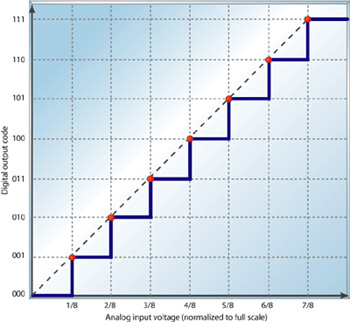
\includegraphics[width=8cm]{22. Arduino mapping}
% \end{wrapfigure}

% De Arduino kan niet alle waarden uitlezen. De ANALOG IN heeft een 10 bits chip. Dit betekent dat er $2^{10} = 1024$ waarden doorgegeven kunnen worden. Het is alsof je de \SI{5.0}{\volt} in 1024 kleine blokjes verdeelt. De waarde die je  uitleest bij opdracht 8 is dus ook niet de spanning zelf, maar het getal dat bij een spanning hoort. Het getal 223 hoort dus bij: $\dfrac{223}{1023} \cdot \SI{5.0}{\volt} = \SI{1.09}{\volt}$ . De PWM ($\sim$) is een 8 bits systeem en kan dus $2^8 = 256$ waarden geven.

% Oei\dots zie je het probleem? We kunnen lezen met 1023 verschillende waardes maar schrijven kan maar met 255 waardes\dots. Gelukkig is er een code die zorgt voor automatische schalen (\lstinline{map}).

% De functie map wil 5 getallen hebben. Het eerste getal is de waarde die de analoge poort uitleest. Het tweede getal is het laagste getal dat uitgelezen kan worden, het derde getal de grootste waarde die uitgelezen kan worden. Dit hoeven niet per se 0 en 1023 te zijn, de waarde verkrijg je bij het ijken van je sensor. De gevoeligheid van je sensor kan dus ook zitten tussen 500 en 900, zie wederom grafiek 2 uit programmeren deel 3. Het vierde en vijfde getal geven het bereik van de output weer. In het voorbeeld moet een input waarde van 500 een output waarde worden van 255. Een input waarde van 900 moet een output waarde van 0 worden.

% \begin{lstlisting}
% void loop() {
%   sensorValue = analogRead(sensorPin);
%   brightness = map(sensorValue,500,900,255,0);
%   Serial.println(sensorValue);
%   delay(10);
%   analogWrite(ledPin,brightness);
% }
% \end{lstlisting}

% \begin{lstlisting}
% void loop(){
%   for(i<5;i++;) {
%     digitalWrite(LEDPin,HIGH);
%     delay(100-i);
%     digitalWrite(LEDPin,LOW);
%     delay(100);
%   }
%   [...]
% }
% \end{lstlisting}

% Een functie die ook handig is, is de functie ++. Elke keer als de loop de volgende cyclus ingaat, wordt de waarde met 1 verhoogd. Zo kun je bijvoorbeeld eenvoudig bijhouden hoeveel loops (iteraties) er al zijn geweest. Ook is het mogelijk om op die manier elke keer een andere pin aan te sturen of later een frequentie te veranderen.

% Als ++ bestaat, dan zal -- ook wel bestaan. En dat klopt. -- zorgt ervoor dat de waarde met 1 wordt verlaagd. Beide codes kunnen in een for-loop geplaatst worden. Dit is een loop binnen de loop. Kijk eens naar het voorbeeld waarbij er een soort aftel mechanisme in zit voordat het programma zelf begint\dots (let op, de variabele i moet je nog wel even declareren voor de setup!

% \subsection{Opdracht 10 Sneller programmeren}

% Herschrijf opdracht 2h met de functie ++.

% \subsection{Opdracht 11 Alarmschakelaar}

% Onder de kassa van een winkel zit een schakelaar (drukknop), als deze wordt ingedrukt dan moet er een pulserend alarmbel (ditmaal nog een LED) gaan. Maak dit systeem.

% \subsection{Opdracht 12 Een RGB LED}

% \begin{wrapfigure}{R}{8cm}
% \raggedleft
% 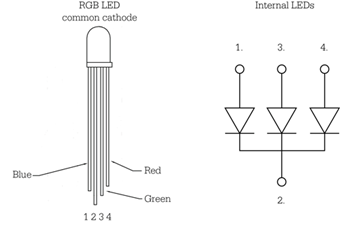
\includegraphics[width=6cm]{23. Component RGB LED}

% 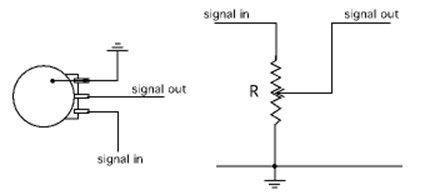
\includegraphics[width=6cm]{24. Component potentiometer}

% 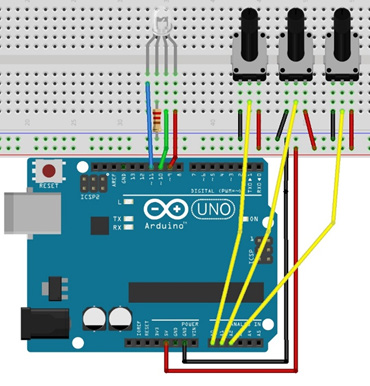
\includegraphics[width=6cm]{25. Circuit RGB LED}
% \end{wrapfigure}

% Een RGB LED heeft vier pootjes. In de LED zitten eigenlijk drie LED’s verwerkt. Door de drie LED’s met behulp van een PWM ($\sim$) aan te sturen kun je kleuren mengen en zo tussenliggende kleuren krijgen. Nu kunnen we via de software de sterkte van elke kleur bepalen, maar het zou leuk zijn wanneer we ook handmatig de kleuren kunnen instellen. We gebruiken hiervoor variabele weerstanden ook wel potmeters genaamd.

% De potmeter heeft drie poten. Eentje voor de \SI{5.0}{\volt} in, eentje voor de aarde (\SI{0.0}{\volt}) en een poot voor het uitlezen van de meter met behulp van een analoge pin, zie ook de figuur hiernaast.

% Als je de draaiknop van de potmeter draait, verandert de weerstand, dit verandert dus ook de waarde van de spanning die je uit leest. Een potmeter is dus eigenlijk een spanningsdeler.

% \begin{enumerate}[label={\alph*})]
% \item Bouw de schakeling.

% \item Schrijf de bijbehorende code waarbij je eerst de waarde van de potmeter uitleest en vervolgens de RGB LED aanstuurt.

% \item Probeer de verschillende standen van de RGB Led en controleer of het plaatje hieronder goed overeenkomt met de kleuren van de LED.
% \end{enumerate}

% 
\includegraphics[width=6cm]{26. Mixing colours}

% \section{Opdracht 13 De snelheid van een elektromotor}

% \begin{wrapfigure}{R}{8cm}
% \raggedleft
% 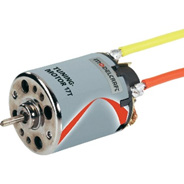
\includegraphics[width=6cm]{27. Component motor}

% 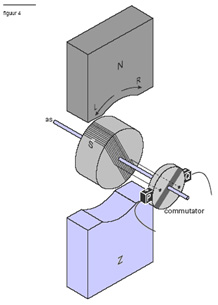
\includegraphics[width=6cm]{28. Component motor schematic}

% 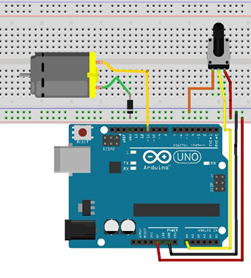
\includegraphics[width=6cm]{29. Circuit motor control}
% \end{wrapfigure}

% Een elektromotor zorgt ervoor dat van elektrische energie bewegingsenergie gemaakt wordt. Een elektromotor vind je in alle apparaten die bewegen en werken op elektriciteit. De snelheid van een elektromotor is afhankelijk van de spanning over de motor. We werken in deze les dus met de PWM pin ($\sim$). We kunnen natuurlijk direct de snelheid van de elektromotor in ons script zetten, maar het zou handiger zijn wanneer we de snelheid van de elektromotor kunnen aanpassen, bijvoorbeeld met behulp van een draaiknop. We gaan gebruik maken van een variabele weerstand, ook wel een potmeter genoemd.

% \begin{enumerate}[label={\alph*})]
% \item Bouw de rechterzijde van de schakeling met de potmeter. De elektromotor hoef je nog niet aan te sluiten.

% \item Leg uit waarom de signal out van de potmeter naar een ANALOG IN moet.

% \item Leg uit waarom de diode is opgenomen in de schakeling.

% \item Programmeer het bijbehorende script zodat de snelheid van draaien van de elektromotor ingesteld kan worden met behulp van de potmeter. Gebruik daarbij de map functie.
% \end{enumerate}

% \section{Elektronica deel 2}

% \begin{wrapfigure}{R}{8cm}
% \raggedleft
% 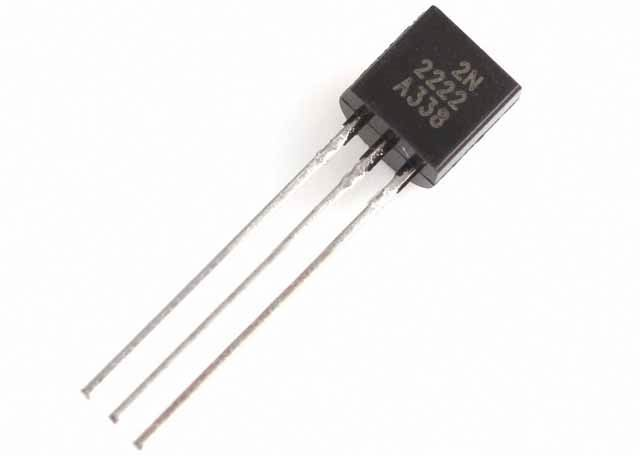
\includegraphics[width=6cm]{30. Component transistor}

% 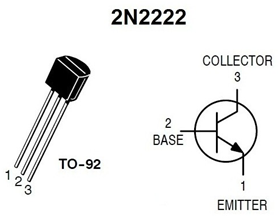
\includegraphics[width=6cm]{31. Component transistor pinout}

% 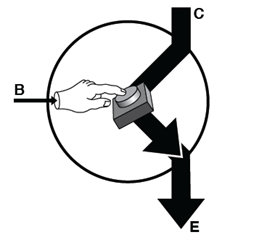
\includegraphics[width=6cm]{32. Component transistor function}
% \end{wrapfigure}

% Een elektromotor kan veel stroom vragen. De Arduino is slecht in het leveren van veel stroom. Om toch grote stroomvragers te voorzien van de benodigde stroom kun je gebruik maken van een externe spanningsbron zoals een batterij. Dan heb je nog wel een transistor nodig zodat je de grootte van de stroom kunt regelen en je de snelheid van draaien van de elektromotor kunt aanpassen.

% De transistor (hier gebruiken we alleen een zogenaamde NPN-transistor) heeft drie pootjes, zie de foto. Links zit de emitter, in het midden de base en aan de rechterzijde de collector. (LET OP! Bij verschillende transistors wordt de volgende omgedraaid, wij hebben de 2N222 transistor). Ten alle tijden wordt aan de collector de externe voeding (+ zijde) verbonden. Spanning over de base bepaalt of er stroom gaat lopen naar de emitter. Daarmee is een transistor een soort van kraan: de hoeveelheid spanning bij de base bepaalt de hoeveelheid doorgelaten stroom. De base moet daarom aangestuurd worden met een PWM pin als je de snelheid wilt regelen.

% Bij erg grote stroomsterktes moet je een grotere transistor gebruiken of eentje met een koelelement zodat de transistor z’n warmte kwijt kan.

% \subsection{Opdracht 14 De snelheid van een elektromotor deel 2}

% \begin{wrapfigure}{R}{12cm}
% \raggedleft
% 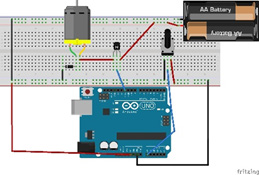
\includegraphics[width=10cm]{33. Circuit motor control (large current)}
% \end{wrapfigure}

% De schakeling van opdracht 13 is te eenvoudig en het kan goed zijn dat de Arduino te weinig stroom levert. Zeker wanneer je de DC motor snel wilt laten draaien.

% \begin{enumerate}[label={\alph*})]
% \item Bouw de schakeling zoals hiernaast weergegeven.

% \item Gebruik het script van opdracht 12 en upload het programma. Kan de elektromotor daadwerkelijk harder draaien?
% \end{enumerate}

% \section{Programmeren deel 4}

% \begin{wrapfigure}{R}{8cm}
% \raggedleft
% 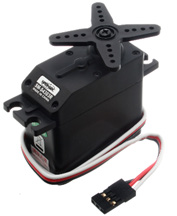
\includegraphics[width=6cm]{34. Component servo}
% \end{wrapfigure}

% Voor het aansturen van sommige apparaten zijn al scripts geschreven waardoor het aansturen van de apparaten eenvoudiger gaat. Een van die apparaten is een servo motor. Een servo motor is een soort elektromotor die 180o kan draaien. De rotatiehoek kan nauwkeurig ingesteld worden doordat deze werkt met een ingebouwde potmeter. Om gebruik te maken van een servo hebben we het volgende script nodig.

% \begin{lstlisting}
% #include <Servo.h>
% Servo mijnServo;
% int pos = 0;
% void setup() {
%   mijnServo.attach(9)
% }
% \end{lstlisting}

% Eerst wordt het script uit de bibliotheek opgehaald. Daarna noemen we de servo mijnServo en krijgt deze de begin positie 0.

% Met \lstinline{mijnServo.attach(9)} zeggen we dat de servo verbonden is met pin 9. Uiteraard is dit weer een PWM poort.

% Nu is het mogelijk de servo te sturen. Waarbij pos staat voor de positie, die kan tussen 0 en 180 zitten. De code voor het sturen van deze servo wordt dan: \lstinline{mijnServo.write(pos);} Een servo motor kan niet helemaal rond draaien zoals een gewone elektromotor maar we kunnen wel heel goed richten met een servomotor. Dit komt omdat er in de Servo een potmeter zit, de sturing gaat dus via het uitlezen van de spanning!


% \section{Opdracht 15 Een lichtwijzer}

% Gebruik opdracht 8 als basis. Vervang daarin de LED door de servo motor. Je kunt op de servo een wijzer plakken en een schaalverdeling maken zodat de wijzer aangeeft hoe licht/donker het is.

% \section{Opdracht 16 Zo veel mogelijk zonlicht}

% \begin{wrapfigure}{R}{8cm}
% \raggedleft
% 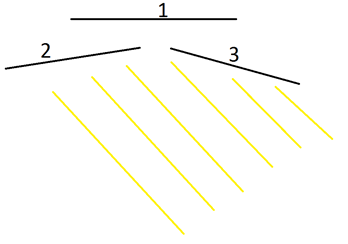
\includegraphics[width=6cm]{35. Control light}
% \end{wrapfigure}

% Zonnepanelen worden neer gezet om stralingsenergie, afkomstig van de zon, om te zetten in elektrische energie. De panelen vangen het meeste licht op als ze loodrecht op de zon staan. De aarde draait en we zouden de panelen mee moeten laten draaien om zoveel mogelijk energie op te vangen. Dat gaan we in deze opdracht doen.

% Op een groot veld staan alle zonnepanelen opgesteld zoals zonnepaneel 1. Zonnepaneel 2 en 3 staan beide een beetje gedraaid ten opzichte van paneel 1. Je kunt nu goed zien dat de zonnepanelen de meeste elektrische energie produceren als zonnepaneel 2 en 3 even veel elektrische energie produceren. Paneel 2 vangt nu meer lichtstralen op dan paneel 3. Het hele systeem zou dus linksom gedraaid moeten worden.

% \begin{wrapfigure}{R}{8cm}
% \raggedleft
% 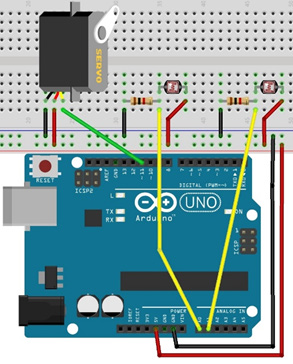
\includegraphics[width=6cm]{36. Circuit solar panel control}
% \end{wrapfigure}

% In plaats van een zonnecel beginnen we met een LDR.

% \begin{enumerate}[label={\alph*})]
% \item Bouw de schakeling en programmeer het eerste stuk waarbij je de waarden van de LDR kan uitlezen.

% \item Zet de flitser van je telefoon aan en lees met behulp van Serial.println(LDR1); de waarden van LDR 1 en LDR2 uit. Beweeg je telefoon van links naar rechts en bekijk hoe de waarden variëren.

% \item Schrijf nu het stukje code voor de servo. Laat de servo naar links draaien als LDR1 meer licht ontvangt dan LDR2 en andersom. Denk eraan dat de servo gebruik maakt van een potmeter en je dus ook gebruik kan maken van de map functie.

% \item Leg uit dat al aardig in de buurt komt van het draaien van de zonnepanelen.
% \end{enumerate}

% \section{Opdracht 17 LCD}

% Met een LCD scherm (liquid cristal display) is het mogelijk om informatie te printen op een klein scherm. Daardoor is het niet meer nodig om gebruik te maken van de seriële monitor (en de computer) om gegevens uit te lezen.

% \begin{minipage}{\textwidth}
% \raggedleft
% 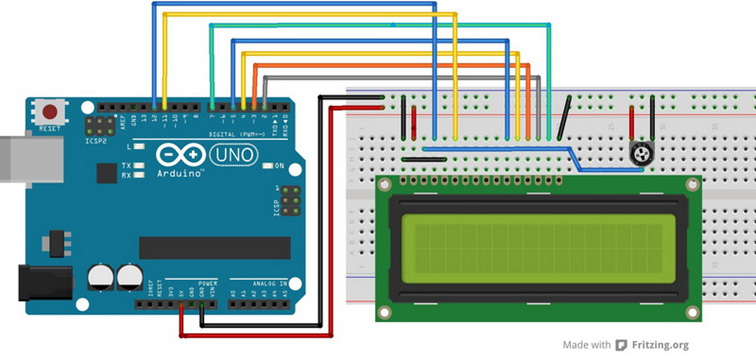
\includegraphics[width=14cm]{37. Circuit display}
% \end{minipage}

% \begin{enumerate}[label={\alph*})]
% \item Maak de opstelling die hier staat.

% \item Open het programma HelloWorld, deze staat bij File/examples/LiquidCrystal en upload het programma. (let op! Bij HelloWorld staat je backlight nog niet aan, deze stuur je met pin 7 (zet het stukje code er in). Je kunt ook de backlight altijd aan hebben, verbind dan niet met pin 7 maar met de +.

% \item Probeer het script te lezen en kijk of je snapt wat de LCD laat zien.
% \end{enumerate}

% Het script maakt gebruik van een library. Een library is een stuk code dat geschreven is door anderen, hierdoor wordt het programmeren je een stuk makkelijker gemaakt. Van heel veel verschillende sensoren zijn al libraries gemaakt, het is dus alleen zaak deze te vinden. Vaak lukt dat wel via bijvoorbeeld instructables.com of arduino.cc. De mogelijke functies staan dan aangegeven. Alle mogelijke functies voor deze library staan op: https://www.arduino.cc/en/ Reference/LiquidCrystal

% Even kijken naar het script: Na het inlezen van de library wijzen we de pinnen aan die gebruikt worden. In de setup wordt aangegeven dat de lcd 16 kolommen en twee rijen heeft (lcd. begin(16,2);).   Ook wordt er meteen de tekst hello, world geprint (alles in de setup wordt 1x gedaan!).

% In de loop wordt de tijd dat de Arduino aan is (millis();) geprint naar de LCD, en wel naar regel 2.

% \begin{enumerate}[label={\alph*})]
% \item Breid je schakeling uit met een drukknop en verander de code zodat het lcd scherm laat zien hoe vaak je op de knop hebt gedrukt.
% \end{enumerate}

% \textbf{Functies}

% Er is een gigantische lijst met functies. Hier de veelgebruikte functies in Arduino.


% \begin{tabular}{p{0.22\textwidth}p{0.78\textwidth}}
% \toprule
% \textbf{Functie} & \textbf{Uitleg} \\
% \midrule
% {\lstinline[]!int!} &
% waarde tussen -32768 en 32767 (215) \\
% {\lstinline[]!long!} &
% waarde tussen -2.147.483.648 en 2.147.483.647 (231) \\
% {\lstinline[]!unsigned long!} / {\lstinline[]!unsigned int!} &
% waardes zijn alleen positief \\
% {\lstinline[]!char!} &
% karakters opgeslagen via het ASCII systeem \\
% {\lstinline[]!float!} &
% zijn decimale waardes, maar wordt zoveel mogelijk omzeild in Arduino programmeertaal \\
% {\lstinline[]!digitalWrite(pin,waarde);!} &
% schrijft geen spanning (LOW) of een spanning van 5 V naar de pin. \\
% {\lstinline[]!analogWrite(pin,waarde)!} &
% schrijft met een 8 bit output waardes tussen 0 en 5 V. De aangegeven waarde moet tussen 0 en 255 liggen. \\
% {\lstinline[]!digitalRead(pin)!} &
% leest of er een spanning op de pin staat, geeft een 0 of 1 terug. \\
% {\lstinline[]!analogRead(pin)!} &
% leest hoeveel spanning op de pin staat, geeft een waarde tussen 0 en 1023 terug. \\
% {\lstinline[]!map(W,Min1,Max1,Min2,Max2)!} &
% Is een schaalfunctie. Converteert een waarde (W) die ligt tussen Min1 en Max1 naar een waarde die ligt tussen Min2 en Max2. \\
% {\lstinline[]!if(voorwaarde){}!} &
% Als er voldaan wordt aan de gestelde voorwaarde, wordt de code tussen de accolades uitgevoerd. \\
% {\lstinline[]!while(voorwaarde){}!} &
% Zolang er aan de voorwaarde voldaan wordt, wordt de code tussen de accolades uitgevoerd. \\
% {\lstinline[]!for(SW;EW;VF){}!} &
% Een for-loop voert de code tussen de accolades een aantal keer uit. SW is de startwaarde, EW de eindwaarde en VF de verhogingsfactor. Vb: {\lstinline[]!for(int i = 0; i<20;i++){delay(100);}!} \\
% {\lstinline[]!switch case!} &
% switch case is een soort keuzemenu waarbij een stukje code uitgevoerd kan worden. Als de variabele waarde een heeft dan voert deze de code uit behorende bij case 1. \\
% {\lstinline[]!&&!} &
% Beide voorwaardes moeten gelden switch \\
% {\lstinline[]!||!} &
% Een van de twee voorwaardes moet gelden \\
% {\lstinline[]!!=!} &
% Is ongelijk aan. \\
% {\lstinline[]!Tone(pin,f,t);!} &
% Kan specifieke frequentie produceren. In de toon moet aangegeven worden op welke pin de luidspreker zit, welke frequentie gemaakt moet worden en eventueel hoe lang de toon aangehouden moet worden. Het is niet noodzakelijk aan te geven hoe lang de toon aangehouden moet worden. \\
% {\lstinline[]!noTone(pin);!} &
% Stopt de toon die geproduceerd werd. \\
% {\lstinline[]!millis();!} &
% Dit kan dienen als een timer. millis(); geeft het aantal milliseconde dat de Arduino aan staat weer. \\
% {\lstinline[]!micros();!} &
% Geeft het aantal microseconde weer dat de Arduino aan staat. De resolutie is \SI{4}{\micro\s}. \\
% {\lstinline[]!delay();!} &
% Wacht een aantal milliseconde voor het uitvoeren van het volgende stukje code. \\
% {\lstinline[]!random(LW,HW)!} &
% Random geeft een getal terug tussen de laagste waarde (LW) en hoogste waarde (HW). Een nadeel van random is dat bij het opnieuw starten van de Arduino dezelfde sequentie wordt afgespeeld. Random is dus niet random\dots Dit probleem kan wel opgelost worden door eerst gebruik te maken van de functie randomSeed(A0); Deze leest pin A0 uit. Als daar niets is verbonden wordt hier ruis gemeten. randomSeed schudt als het ware de vaste sequentie van Random door elkaar.\\
% \bottomrule
% \end{tabular}


% \begin{lstlisting}
% (var) {
%   case 1: //doe iets als var is 1
%   break;
%   case 2: //doe iets als var is 2
%   break;
%   default: // als geen van bovenstaande waar is, doe het volgende (optioneel)
%   break;
% }
% \end{lstlisting}

\end{document}